

\documentclass{article}
\author {Yuke Chen, Yixiang Gong, Tiffani Rachman, Kensuke Tamura, Tudor Vasile, Tudor Zugravu}
\title{Kings College London \\ Group Project  (7CCSMGPR).  \\ Initial Report} 
\usepackage{a4wide}
\usepackage{graphicx}
\usepackage{float}
\usepackage{multirow}

\begin{document}

	\maketitle
	\pagenumbering{roman}


	\paragraph{}
	\fontsize{12}{12}\selectfont
	
	\section{Project description}
	Team kchat has been assigned to create a multi-user chat application. The system will be designed as a three-tier architecture model, being comprised of a server side, a central database and client user interface. In order to cover the most used platforms today, the system provides Android, iOS mobile interfaces and a web platform.\\
	
	\textbf{Priority aims:}\\
	
	Our first aim is to configure the server side of our system, allowing bidirectional connections with external entities. This is achieved by implementing the server side in Node.js, a JavaScript runtime environment and through using Socket.IO, a JavaScript library. The main advantage of these technologies is to provide a real-time event-based communication between the server and clients. In addition, Node.js's design allows us to create the system as a scalable network application, providing the means to use cloud computing technologies. \\\par
	The second aim is to design the central database on the server based upon the data required by our system. This component will be planned as a relational database and will be manipulated using MySQL through phpMyAdmin. All data such as user's information, the sent messages and chat rooms will be stored in the central database. However, the mobile applications will make use of internal databases in order to store user-specific data and recent messages. The amount of data that can be stored on the device will be restricted in order not to overload the memory and to avoid crashes due to storage limitations (Android applications are limited to 100MB of memory).\\\par
	An important part of this project is the development of mobile applications on both Android and iOS operating systems. As soon as implementation starts, the connection to the central server will be established in order to download the necessary information such as available chat rooms, online users and incoming messages. The receival of messages can be achieved either by using the bidirectional communication when the apps are active or through push notifications when they are suspended. \\\par
	The web interface will also communicate through the use of sockets. However, it will only operate with the main database, as the connection will be maintained throughout the whole period and active-user-specific information will be stored in sessions. The features provided by the web interface will be the same as the ones from the mobile applications. \\\par
	In order to achieve a large coverage of potential users, the system will target a large number of devices by meeting the requirements of the most frequently used mobile operating systems (iOS 8.0 - iOS 10.0 and Android 4.4 - Android 7.0). In addition, the web platform will target the most used web browsers (Google Chrome, Safari, Internet Explorer and Mozilla Firefox). \\\par
	After registration, the users will have to log in to use the system. A profile management section is provided, where the user can change the profile picture and specific information can be set. The user should be able to create private/public rooms that can also be used as one-to-one conversations. In addition, he can leave groups, ban groups from his list and manage his contact list.  \\\par
	Graphical User Interface rules will be clearly stated in order to provide consistency between client systems. The mobile applications will follow the same design, whereas the web platform will have a different layout, but will respect the design and colour schemes. \\\par
	
	\textbf{Optional Aims} \\ \newline
	Certain features have been categorised as optional, the main aim being to develop a working chat system on multiple devices. However, if there are enough time resources left, a number of desired features will be implemented as well. Such an optional aim is to provide image and video transfers sent from clients to the server. In order to achieve this, the sent images will have to be scalled down and to set a limit on the size of transmitted media files.\\ \par
	Another aim is introducing security features such as message encryption on transmission and full encryption of the database for each android device. This can be achieved by using a standard hash function (MD-5) and possibly include a salt for strengthened security.\\ \par
	Aditional features include different permissions for the type of users. In addition to the standard user options, the admin should also be able to blacklist users who are not following the correct rules or are causing harm to the system in certain ways.   \newline
	\newpage
	
    \section{Project Organisation}
	Our team decided to adapt the agile software methodology. Early on in the process, we decided to use online project management tools which allows us to communicate and host our workloads. Technologies such as Trello (https://trello.com/b/FHlyPkTd/kchat) have been used where the projects backlog is contained. These also include updates on our roles where the backlog is reduced during each sprint iteration. It is important to note that the backlog can change in a sprint environment, so new tasks could be added at any time.  Our team has also created a roadmap for each sub team with the list of priority tasks and a time to finish them by. To deviate from the social side of Facebook communication, our team is using Slack (https://slack.com/). This technology allows us to communicate with the use of sub-channels to stay organised.\\ \par 
	We decided as a team to break down into 3 groups where all of us would program one platform of the chat system. Groups were divided to suit our skillsets and knowledge where each member chose freely the group they most feel comfortable in. Overall, we have 3 subgroups consisting of team Android, IOS and Web. Our aim is to complete the work required for one technology and then move around helping the other teams when needed. In addition, we all contribute to the system's server implementation and participate in the project management side.\\ \par 
	
	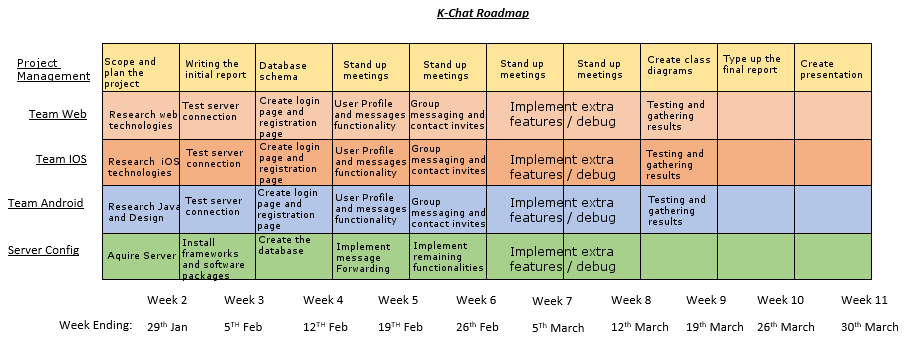
\includegraphics[width=\textwidth]{roadmapkchat.png}
	
	We also make use of retrospectives where we reflect weekly on what work was completed successfuly and what tasks have encountered problems. Rather than individually criticising each member, we learn from our retrospectives as a team, in order to build on our weaknesses.\\ \par 
	Each team member can easily report back if they have conflicts, find the work not interesting or too difficult and we would then try to support each other by either helping out with providing ideas or assisting in solving the problem. In the worst case, members can be swapped to work on other programming technologies.
	
	
	
	
	
	
\end{document}






